\begin{table}[h]
\centering
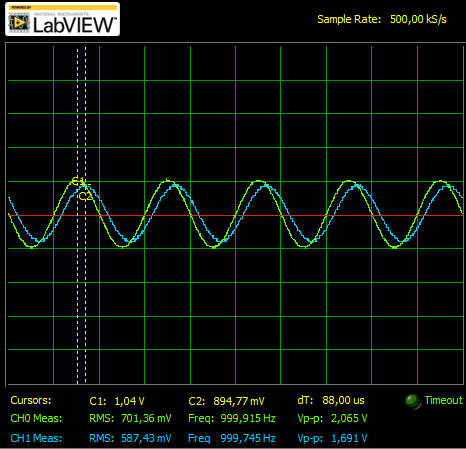
\includegraphics[scale=0.7]{graficos/RGADICOA1}
\end{table}
\begin{center}
Gráfico 2: Resposta para Frequência 1kHz
\end{center}


\begin{table}[h]
\centering
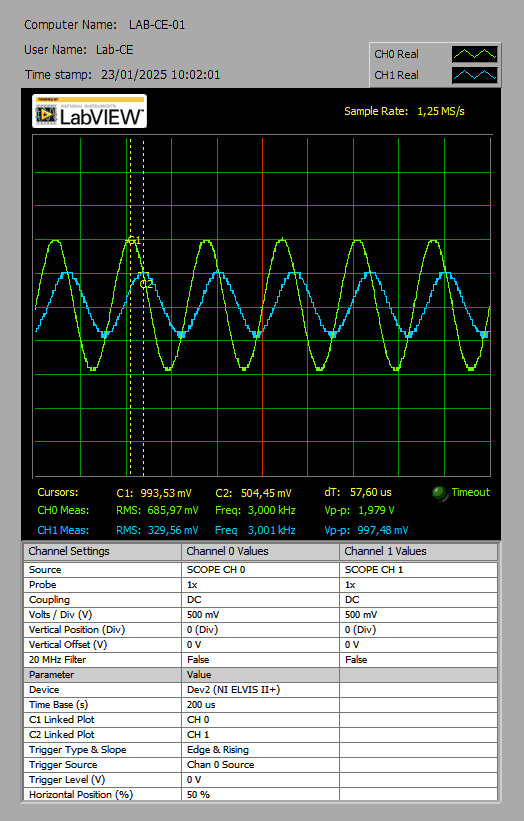
\includegraphics[scale=0.7]{graficos/RGADICOA3}
\end{table}
\begin{center}
Gráfico 3: Resposta para Frequência 3kHz
\end{center}

\newpage
\begin{table}[h]
\centering
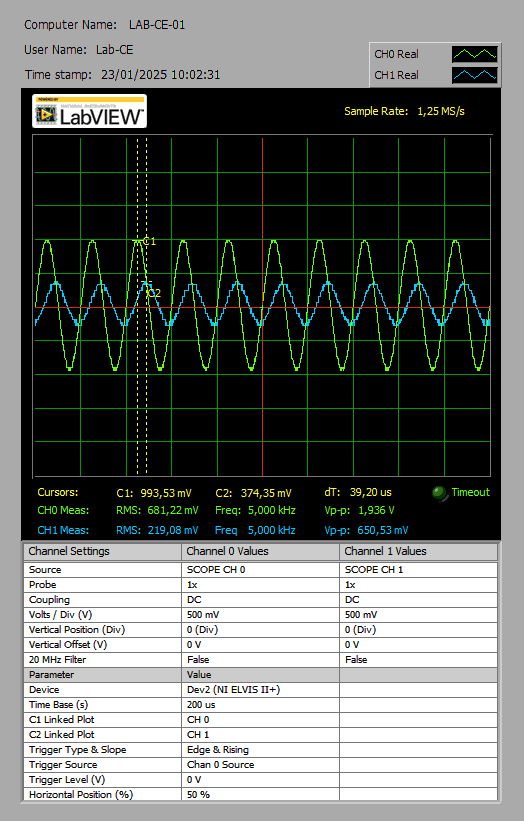
\includegraphics[scale=0.7]{graficos/RGADICOA5}
\end{table}
\begin{center}
Gráfico 4: Resposta para Frequência 5kHz
\end{center}


\begin{table}[h]
\centering
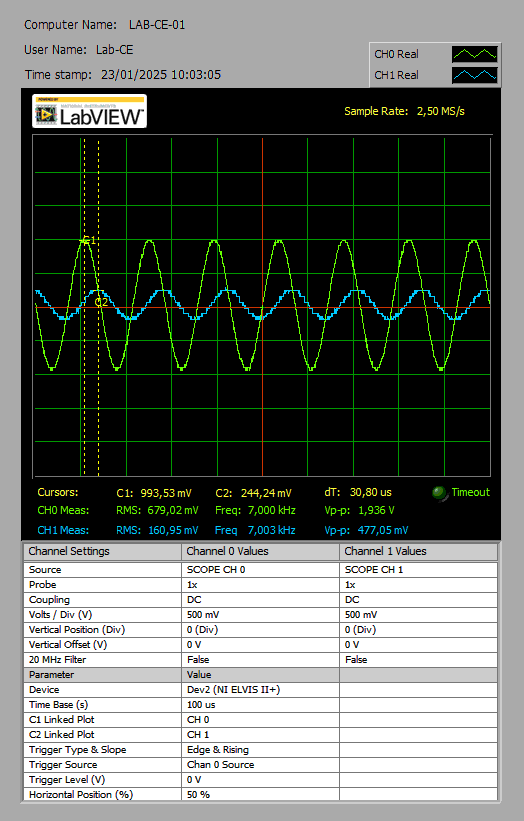
\includegraphics[scale=0.7]{graficos/RGADICOA7}
\end{table}
\begin{center}
Gráfico 5: Resposta para Frequência 7kHz
\end{center}

\newpage
\begin{table}[h]
\centering
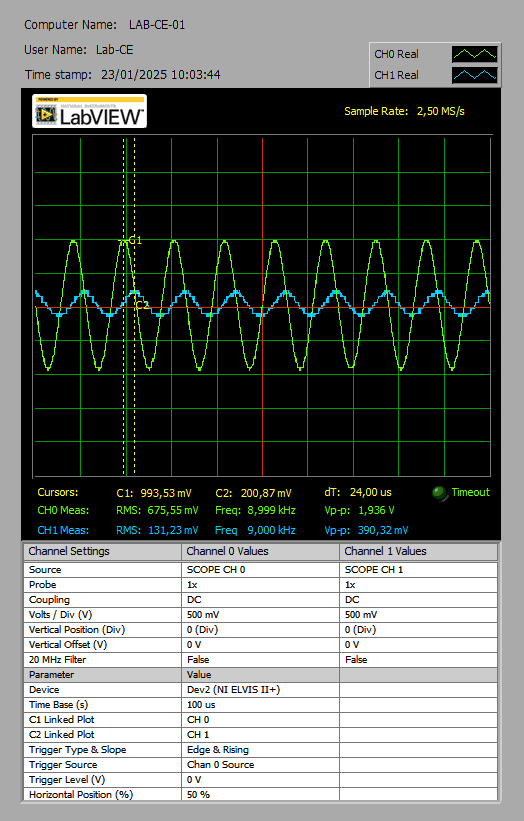
\includegraphics[scale=0.7]{graficos/RGADICOA9}
\end{table}
\begin{center}
Gráfico 6: Resposta para Frequência 9kHz
\end{center}


\begin{table}[h]
\centering
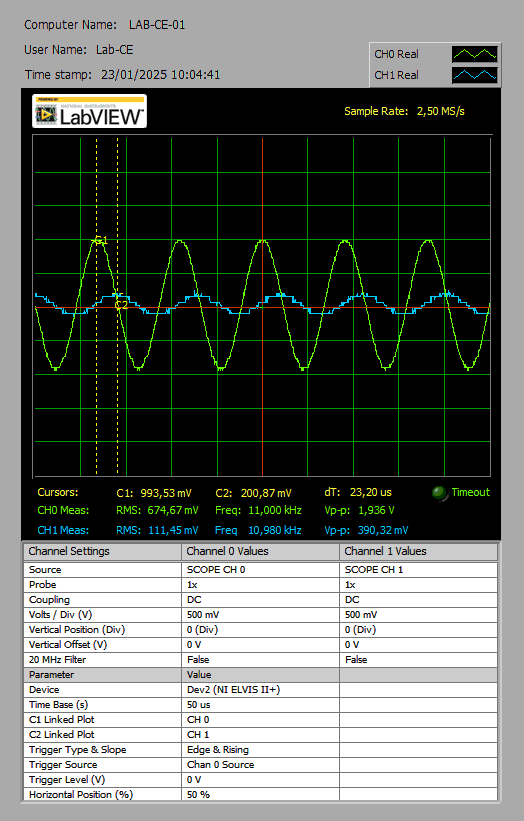
\includegraphics[scale=0.7]{graficos/RGADICOA11}
\end{table}
\begin{center}
Gráfico 7: Resposta para Frequência 11kHz
\end{center}

\newpage
\begin{table}[h]
\centering
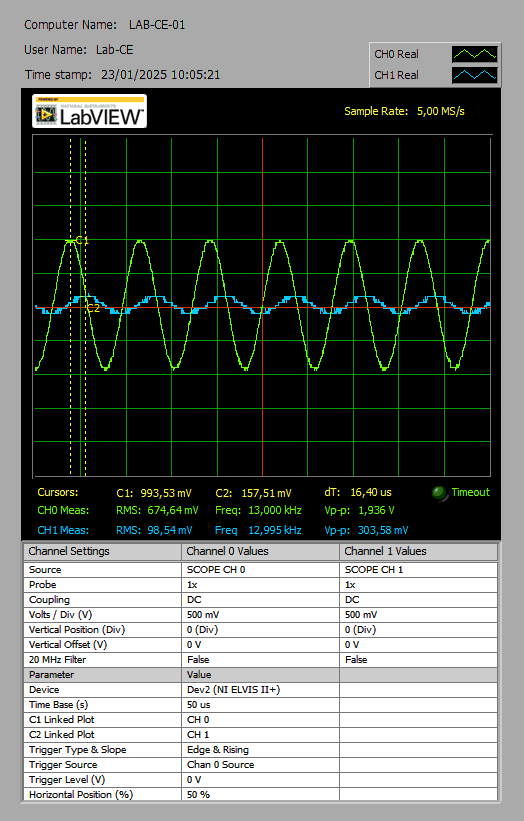
\includegraphics[scale=0.7]{graficos/RGADICOA13}
\end{table}
\begin{center}
Gráfico 8: Resposta para Frequência 13kHz
\end{center}


\begin{table}[h]
\centering
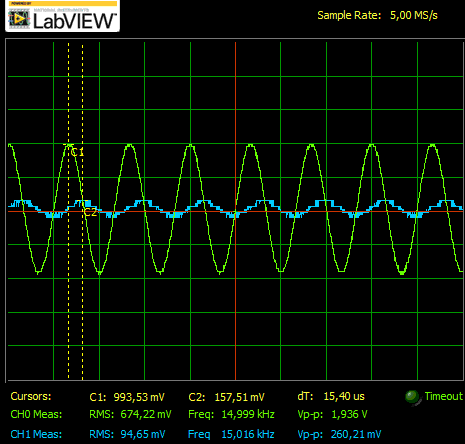
\includegraphics[scale=0.7]{graficos/RGADICOA15}
\end{table}
\begin{center}
Gráfico 9: Resposta para Frequência 15kHz
\end{center}

\newpage
\begin{table}[h]
\centering
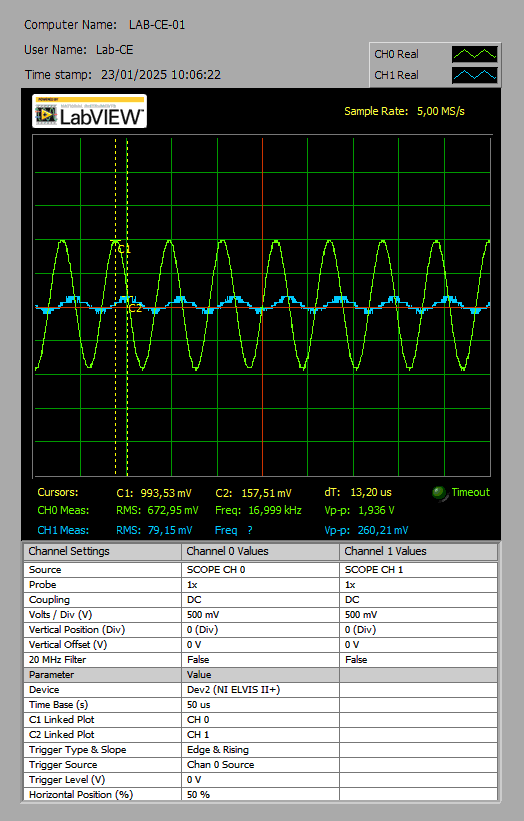
\includegraphics[scale=0.7]{graficos/RGADICOA17}
\end{table}
\begin{center}
Gráfico 10: Resposta para Frequência 17kHz
\end{center}


\begin{table}[h]
\centering
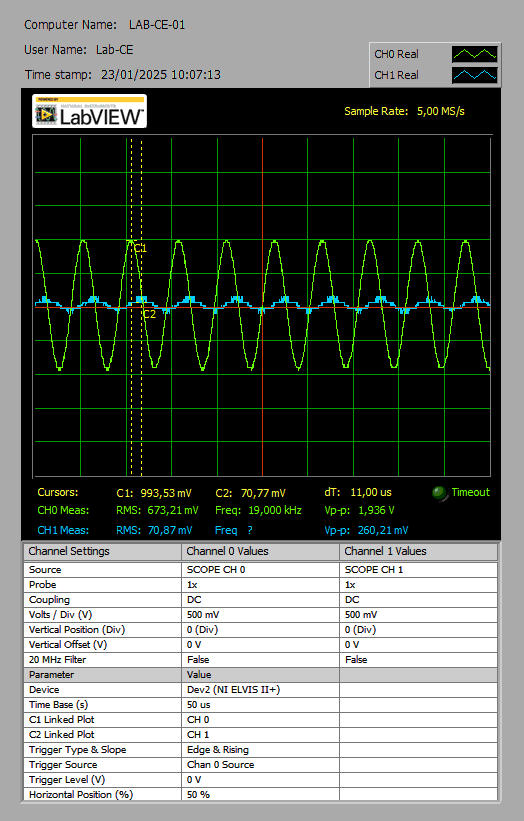
\includegraphics[scale=0.7]{graficos/RGADICOA19}
\end{table}
\begin{center}
Gráfico 11: Resposta para Frequência 19kHz
\end{center}